\documentclass{beamer}
\usepackage{amsfonts,amsmath,oldgerm}
\usepackage{tabularx, booktabs, multirow, siunitx}
\usepackage{ragged2e}
\justifying
\usetheme{sintef}
\usepackage{tikz}
\usetikzlibrary{arrows.meta,positioning,calc,fit,backgrounds,decorations.pathreplacing}
\usepackage{adjustbox}
% ------------------------------------------------------------------ styles

\definecolor{hostc}{HTML}{DCE8F5}
\definecolor{devc}{HTML}{FBE3C8}
\definecolor{memc}{HTML}{DDF0DA}
\definecolor{padc}{HTML}{D9D9D9}
\definecolor{lA}{HTML}{8DB6E0}
\definecolor{lB}{HTML}{F2B880}
\definecolor{lC}{HTML}{9CCF95}
\definecolor{lD}{HTML}{E59A9A}
\definecolor{lE}{HTML}{C3A7DB}
\definecolor{lF}{HTML}{E8D98A}
\tikzset{
  dbox/.style={draw,rounded corners=2pt,align=center,font=\small,inner sep=4pt,fill=devc},
  hbox/.style={draw,rounded corners=2pt,align=center,font=\small,inner sep=4pt,fill=hostc},
  mbox/.style={draw,rounded corners=2pt,align=center,font=\small,inner sep=4pt,fill=memc},
  darr/.style={-{Latex[length=2mm]},thick},
  sectag/.style={font=\sffamily\scriptsize,fill=white,draw=gray,rounded corners=1pt,inner sep=1.5pt},
}



% Roadmap of the design steps; #1 = highlighted step (0 = none)
\newcommand{\roadmap}[1]{%
\begin{center}
\begin{tikzpicture}[x=1cm,y=1cm,font=\scriptsize]
\foreach \i/\name/\where in {1/Data layout/device, 2/Coarse search/device,
   3/List union/host, 4/Scheduling/host, 5/Fine search/device,
   6/Top-$k$ merge/device, 7/Multi-batch/device}{
  \ifnum\i=#1
    \node[draw=maincolor,fill=maincolor,text=white,font=\scriptsize\bfseries,
          rounded corners=2pt,minimum width=1.72cm,minimum height=0.62cm,align=center]
          (r\i) at (\i*1.95,0) {\name};
  \else
    \node[draw=gray!60,fill=gray!12,text=gray!70!black,
          rounded corners=2pt,minimum width=1.72cm,minimum height=0.62cm,align=center]
          (r\i) at (\i*1.95,0) {\name};
  \fi
  \node[font=\tiny,text=gray] at (\i*1.95,-0.48) {\where};
}
\foreach \i [evaluate=\i as \j using int(\i+1)] in {1,...,6}{
  \draw[-{Latex[length=1.4mm]},gray!70] (r\i.east) -- (r\j.west);}
\end{tikzpicture}
\end{center}\vspace{-2mm}}
% figure that fits the remaining space
\newcommand{\slidefig}[2][0.62]{\begin{adjustbox}{max width=\linewidth,max height=#1\textheight,center}\input{src/figs/#2}\end{adjustbox}}


\usefonttheme[onlymath]{serif}

\titlebackground*{assets/background}

\newcommand{\hrefcol}[2]{\textcolor{cyan}{\href{#1}{#2}}}

% Figures: slide-specific images first, then the thesis figures
\graphicspath{{images/}{../src/assets/}}

\title{Approximate Nearest-Neighbor Search on the Tenstorrent Wormhole Architecture}
\course{Master's Degree in Computer Science}
\author{\href{mailto:Barbalata.2002688@studenti.uniroma1.it}{Barbalata Radu Ionut}}
\IDnumber{2002688}
\date{Academic Year 2025/2026}

\begin{document}
\maketitle

\section{Introduction}

\begin{frame}{Motivation}
  \begin{itemize}
    \item Vector search retrieves the items most similar to a query embedding: it is the retrieval step of RAG, recommendation, and semantic search
    \item Exact search compares the query with every vector: too slow for large collections
    \item Approximate nearest-neighbor (ANN) indexes trade a little recall for much higher speed
    \item Today ANN search runs on CPUs and GPUs
    \item \textbf{Tenstorrent} builds tile-based AI accelerators: can they also serve vector search, and at what performance and energy cost?
  \end{itemize}
\end{frame}

\begin{frame}{Research Questions}
  \begin{enumerate}
    \item Which ANN index structure suits the Tenstorrent architecture and programming model?
    \item Can an IVF-based pipeline be implemented efficiently with tiles, explicit data movement, and distributed Tensix cores?
    \item What Recall@10 and throughput does it reach compared with multicore CPUs and an NVIDIA A100?
    \item How does its energy compare at matched recall?
  \end{enumerate}
\end{frame}

\begin{frame}{Contributions}
  \begin{itemize}
    \item Analysis of the main ANN index families for Tenstorrent $\Rightarrow$ IVF-Flat
    \item First ANN implementation on Tenstorrent, on a Wormhole n150
    \item Comparison with Faiss on 56/112 CPU cores and an A100 at matched Recall@10
    \item Throughput, workload energy, and a stage-level analysis of the bottlenecks
  \end{itemize}
\end{frame}

\section{Background}

\begin{frame}{Approximate Nearest-Neighbor Search}
  \begin{itemize}
    \item Database of $n$ vectors in $\mathbb{R}^d$, query $q$: find the $k$ most similar vectors
    \item Similarity: inner product on normalized vectors (cosine)
    \item Quality measured by \textbf{Recall@10}: fraction of the true 10 nearest neighbors that are returned
    \item Main index families: inverted files (IVF), graphs (HNSW, CAGRA), quantization (IVF-PQ, ScaNN)
  \end{itemize}
\end{frame}

\begin{frame}{Inverted File Index (IVF)}
  \begin{columns}
    \column{0.5\textwidth}
    \begin{itemize}
      \item $k$-means splits the database into $N_{\mathrm{list}}$ cells
      \item \textbf{Coarse search:} compare the query with all centroids
      \item \textbf{Fine search:} scan only the $N_{\mathrm{probe}}$ closest lists
      \item Larger $N_{\mathrm{probe}}$: higher recall, more work
    \end{itemize}
    \column{0.5\textwidth}
    \centering
    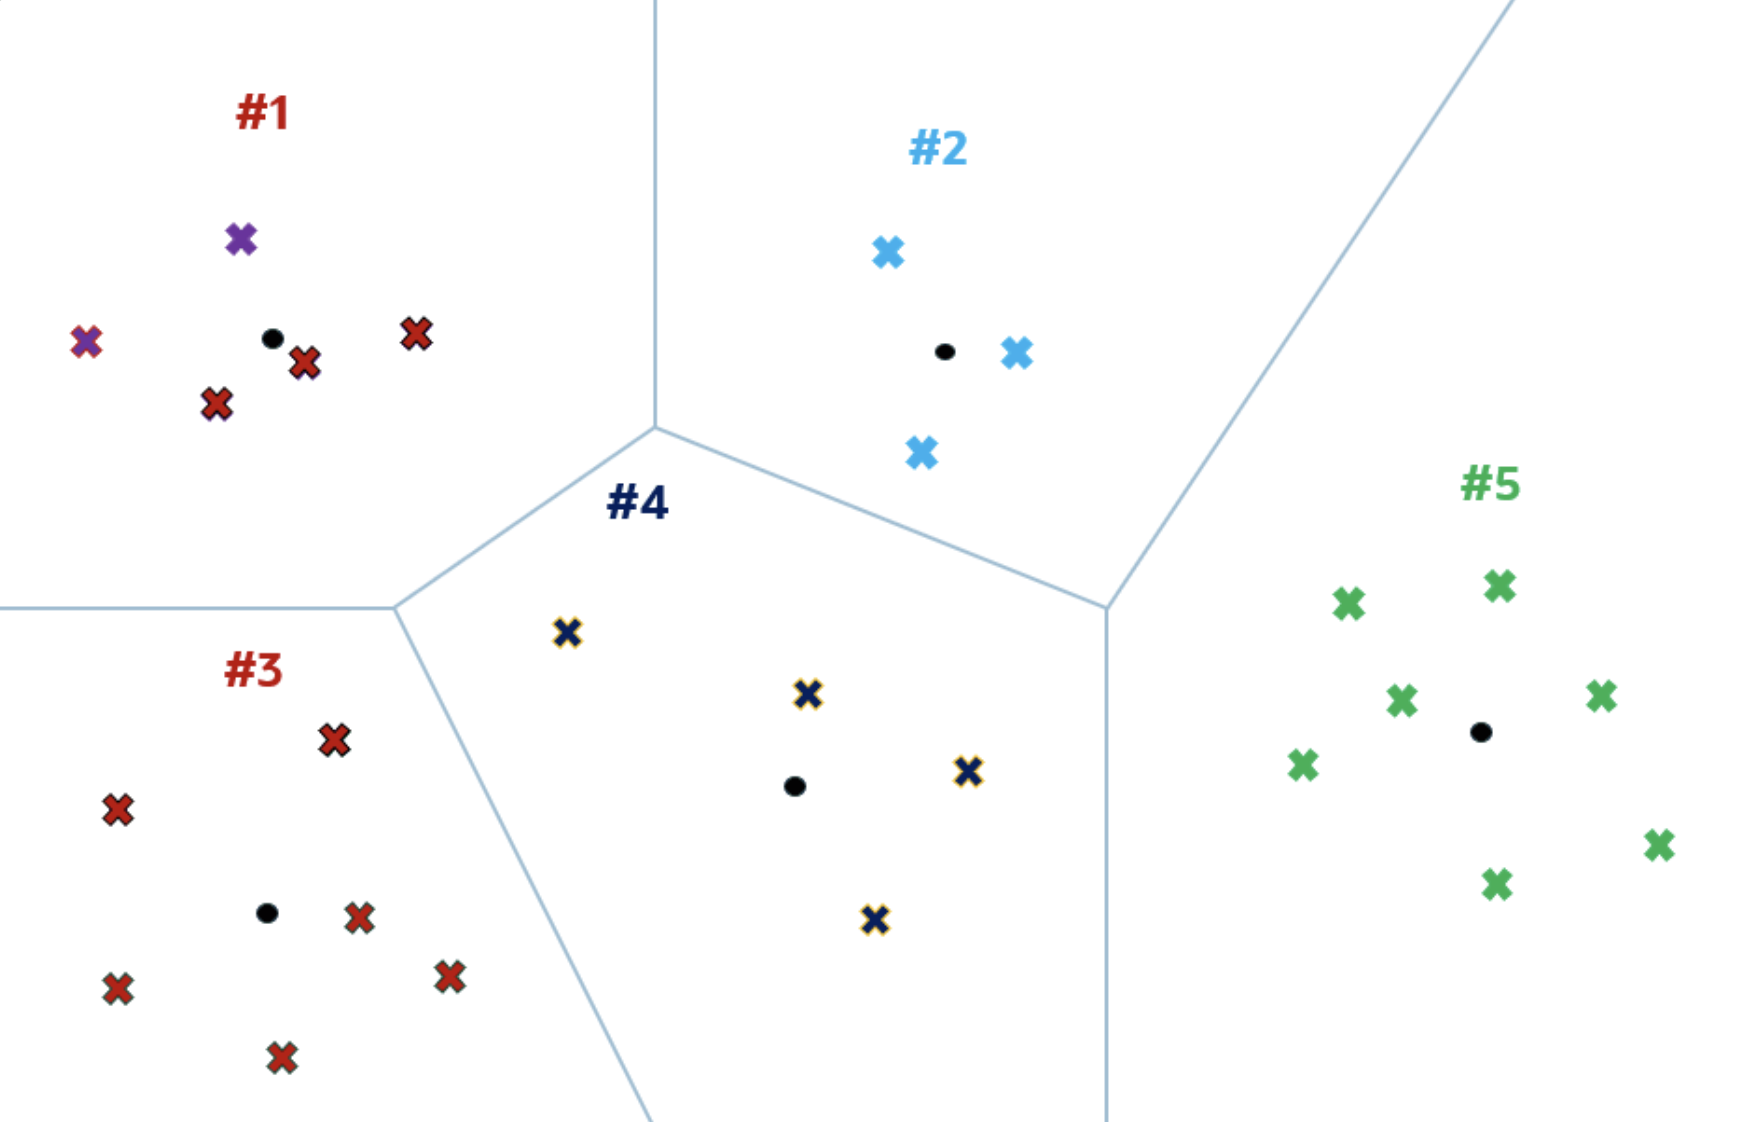
\includegraphics[width=\linewidth]{voronoi_cells.png}
  \end{columns}
\end{frame}

\begin{frame}{Why Approximate: Missed Neighbors}
  \centering
  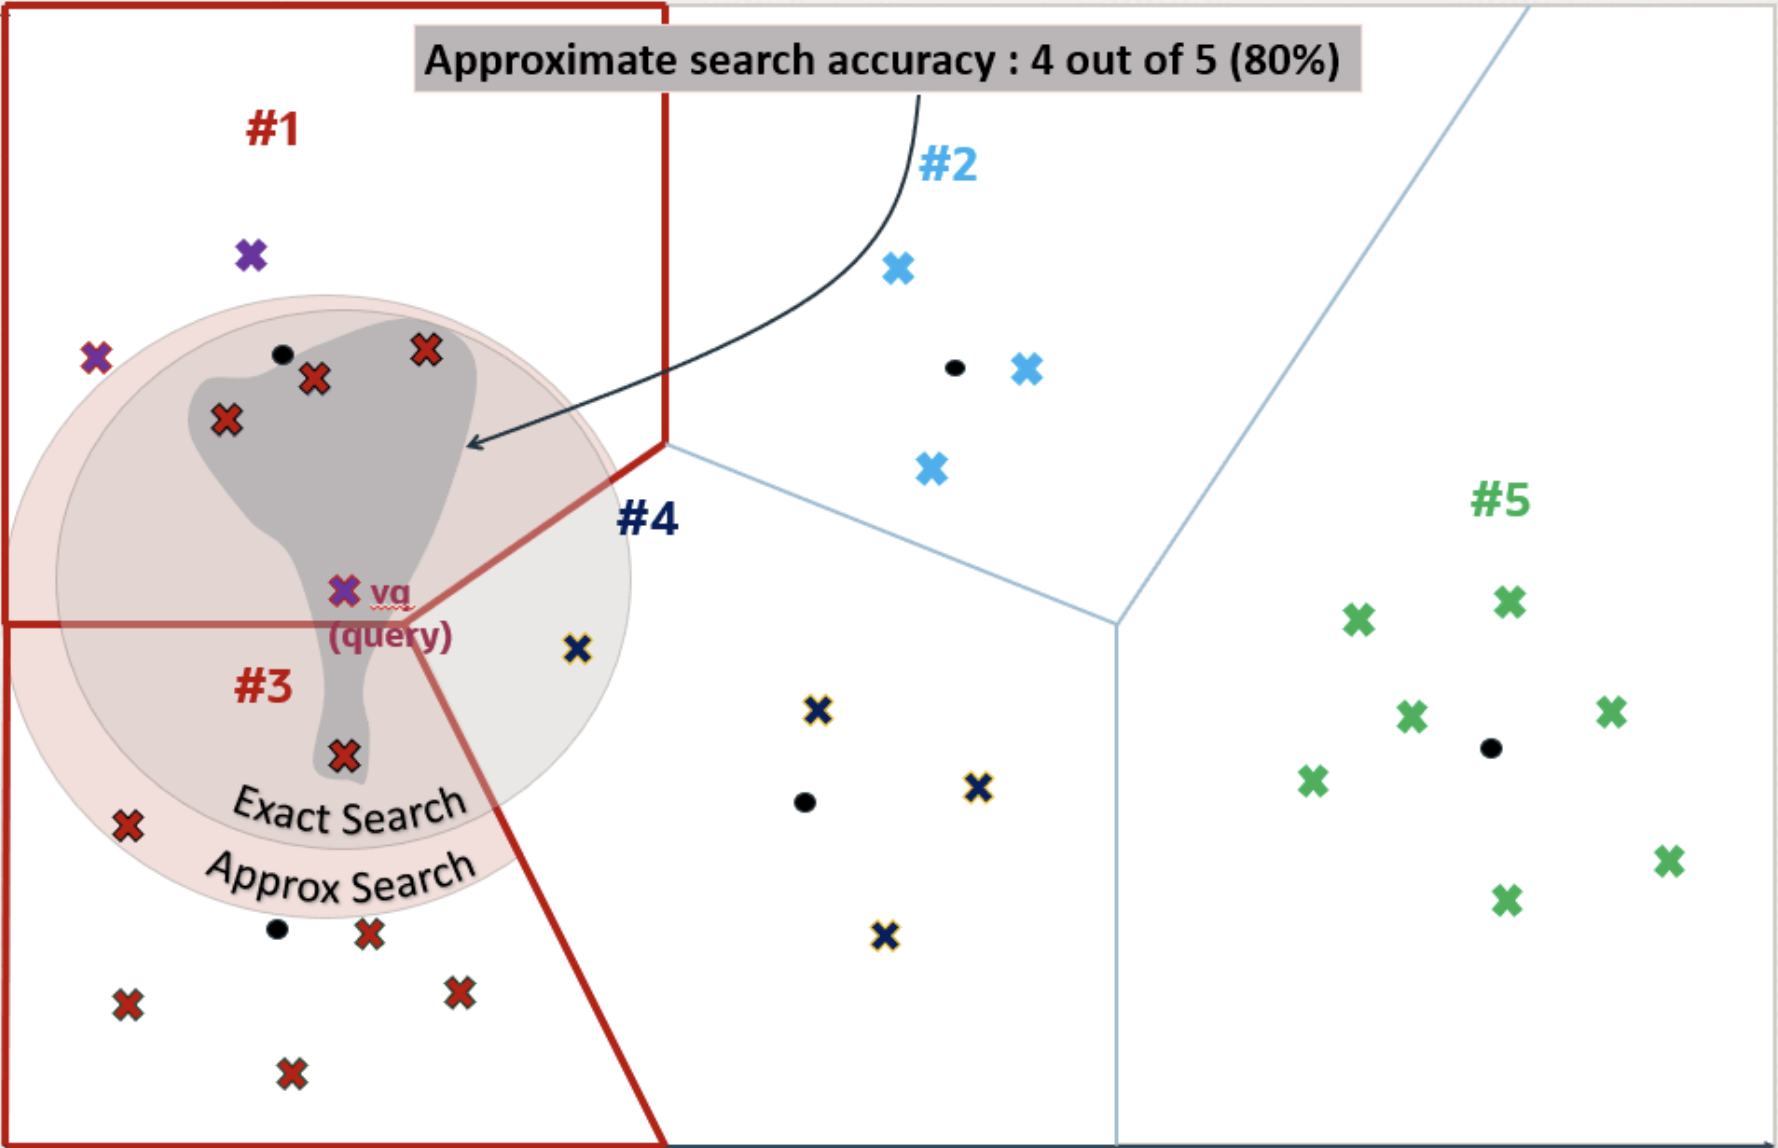
\includegraphics[height=0.68\textheight]{ivf_missed_vector.png}\\[1mm]
  {\footnotesize A true neighbor in an unprobed cell is missed: $N_{\mathrm{probe}}$ trades recall for speed}
\end{frame}

\begin{frame}{Tenstorrent Wormhole n150}
  \begin{columns}
    \column{0.5\textwidth}
    \begin{itemize}
      \item Grid of Tensix cores connected by a network-on-chip (NoC)
      \item Each core: five RISC-V cores, local L1 SRAM, matrix engine on $32\times32$ tiles
      \item 12\,GB GDDR6 device DRAM, attached via PCIe
      \item TT-Metalium: reader, compute, and writer kernels linked by circular buffers
    \end{itemize}
    \column{0.5\textwidth}
    \centering
    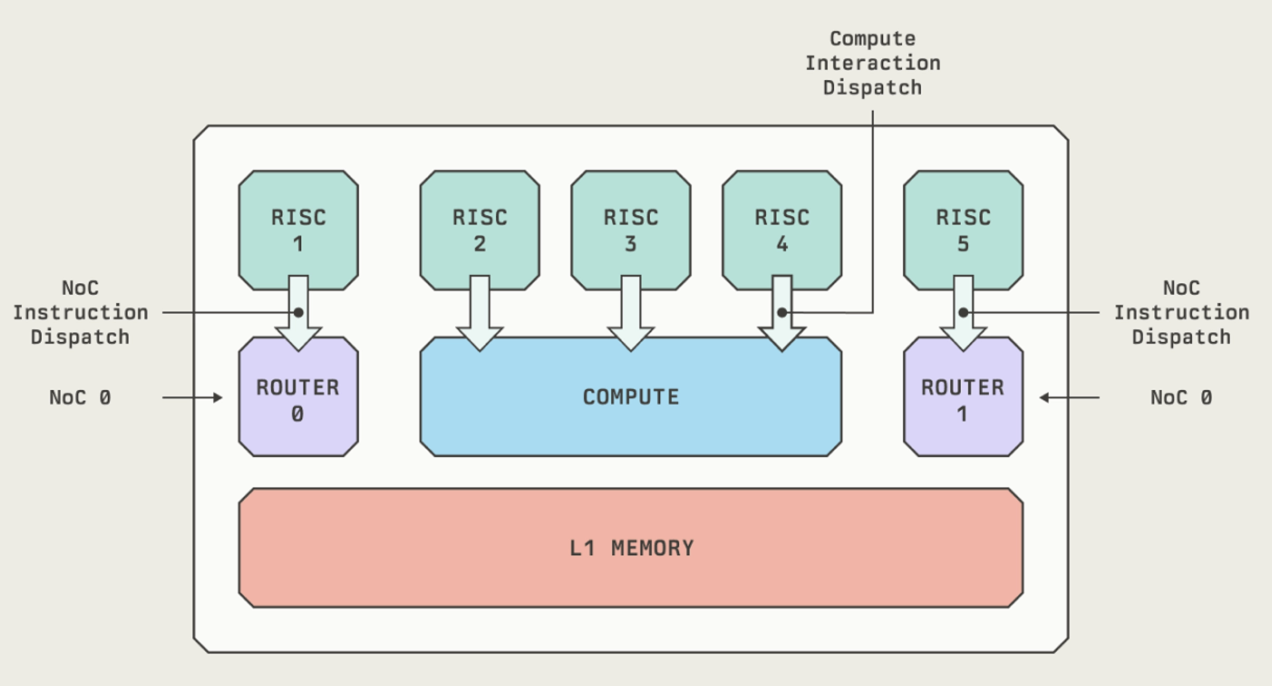
\includegraphics[width=\linewidth]{tensix.png}
  \end{columns}
\end{frame}

\begin{frame}{Why IVF-Flat?}
  \begin{itemize}
    \item \textbf{Graphs} (HNSW, CAGRA): irregular, data-dependent traversal, poor fit for tiles
    \item \textbf{Quantization} (IVF-PQ, ScaNN): codebook lookups map poorly onto the matrix engine
    \item \textbf{IVF-Flat}: dense products between query tiles and contiguous lists
    \begin{itemize}
      \item regular, fixed-shape computation
      \item predictable, streamable memory access
      \item the irregular part (list selection) can be handled on the host
    \end{itemize}
  \end{itemize}
\end{frame}

\section{Design and Implementation}

\begin{frame}{Overview}
  \roadmap{0}
  \slidefig[0.66]{map}
\end{frame}

\begin{frame}{Running Example}
  \roadmap{0}
  \centering\footnotesize
  \begin{tabular}{lcc}
    \toprule
    & Example & Implementation \\
    \midrule
    Tile size & $4\times4$ & $32\times32$ \\
    Queries per batch & 4 ($q_0$--$q_3$) & 32 \\
    Inverted lists & 8 (A--H) & 512--2048 \\
    Lists per query $N_{\mathrm{probe}}$ & 2 & 1--32 \\
    Top-$k$ state & top-2 & top-32 \\
    Fine-search workers & 3 (W1--W3) & 63 \\
    Chunk limit & 2 pages & 128 pages \\
    \bottomrule
  \end{tabular}\\[2mm]
  Selections: $q_0$\{A,\,C\}, $q_1$\{A,\,B\}, $q_2$\{C,\,E\}, $q_3$\{A,\,D\}
\end{frame}

\begin{frame}{Step 1: Tiled Data Layout}
  \roadmap{1}
  \slidefig[0.3]{layout}
  \begin{itemize}\footnotesize
    \item Lists stored as \textbf{pages} of 32 vectors, dimensions padded to multiples of 32 (100 $\to$ 128)
    \item Each page has an identifier tile; padded slots carry a sentinel and are masked to $-10000$
    \item Index uploaded once to device DRAM; packed buffers addressed by page offset
  \end{itemize}
\end{frame}

\begin{frame}{Step 1: Query Batch $\times$ Page}
  \roadmap{1}
  \slidefig[0.32]{batchpage}
  \begin{itemize}\footnotesize
    \item A batch of 32 queries is the row operand, a page of 32 vectors the column operand
    \item One tile product scores every query of the batch against every vector of the page
  \end{itemize}
\end{frame}

\begin{frame}{Step 2: Coarse Search}
  \roadmap{2}
  \begin{columns}
    \column{0.62\textwidth}
    \slidefig[0.58]{coarse}
    \column{0.38\textwidth}
    \begin{itemize}\footnotesize
      \item Regular, dense: runs on the device
      \item Query tiles stay in L1, centroid blocks of 32 streamed from DRAM
      \item Running top-32 per query, so $N_{\mathrm{probe}}\le32$
      \item Example: E replaces D for $q_2$ in block 2
    \end{itemize}
  \end{columns}
\end{frame}

\begin{frame}{Step 3: Batch-Level List Union}
  \roadmap{3}
  \begin{itemize}
    \item The host collects the lists selected by all queries of a batch into one set
    \item[] \centering $\mathcal{U}_b=\bigcup_{r} \mathcal{P}_{b,r}$ \quad e.g.\ 8 selections $\to$ $\{$A,B,C,D,E$\}$
    \item Why: a page costs one tile product whether 1 or 32 queries need it
    \item Consequence: each query is also scored against the lists of the other queries
    \item With queries in dataset order, batches share few lists: each query scans \textbf{12--32$\times$} the vectors of its own lists
  \end{itemize}
\end{frame}

\begin{frame}{Step 4: Scheduling on 63 Workers}
  \roadmap{4}
  \begin{columns}
    \column{0.58\textwidth}
    \slidefig[0.55]{schedule}
    \column{0.42\textwidth}
    \begin{itemize}\footnotesize
      \item Lists longer than 128 pages split into chunks
      \item Weight = number of pages
      \item LPT: longest task to the least-loaded worker
      \item One description per worker in DRAM: (offset, page count) per task
      \item Host cost: at most 3\% of search time
    \end{itemize}
  \end{columns}
\end{frame}

\begin{frame}{Step 5: Fine Search -- Data Movement}
  \roadmap{5}
  \slidefig[0.5]{datamovement}
  \begin{itemize}\footnotesize
    \item Reader (NCRISC) streams pages over the NoC, double-buffered
    \item Compute (TRISC0--2) scores the page; writer (BRISC) stages results in DRAM
  \end{itemize}
\end{frame}

\begin{frame}{Step 5: Fine Search -- One Page}
  \roadmap{5}
  \slidefig[0.36]{page}
  \begin{itemize}\footnotesize
    \item Multiply the query tiles by the page: one $32\times32$ score tile
    \item Last page of a list: padded slots recognized by their sentinel ID and set to $-10000$
    \item Scores merged into the running top-32 of each query
  \end{itemize}
\end{frame}

\begin{frame}{Step 5: Fine Search -- Top-32 Update}
  \roadmap{5}
  \slidefig[0.5]{localtopk}
  \begin{itemize}\footnotesize
    \item Only the current page is transposed; the saved state is already kept transposed
    \item \texttt{topk\_local\_sort} orders each query column and moves scores and IDs together
  \end{itemize}
\end{frame}

\begin{frame}{Step 6: Hierarchical Top-$k$}
  \roadmap{6}
  \begin{columns}
    \column{0.6\textwidth}
    \slidefig[0.58]{staging}
    \column{0.4\textwidth}
    \begin{itemize}\footnotesize
      \item Each worker writes its partial top-32 to its own DRAM slot
      \item Completion semaphore on core $(0,0)$; ready semaphore back to each worker
      \item Core $(0,0)$ merges all slots: \textbf{final top-32 on the device}
      \item Host only reads it and keeps $k$
    \end{itemize}
  \end{columns}
\end{frame}

\begin{frame}{Step 7: Multi-Batch Execution}
  \roadmap{7}
  \slidefig[0.42]{multibatch}
  \begin{itemize}\footnotesize
    \item All batches of a workload run in one coarse and one fine invocation
    \item Workers continue with the next batch; aggregation follows behind
    \item Launch, synchronization, and host orchestration amortized over many batches
  \end{itemize}
\end{frame}

\section{Methodology}

\begin{frame}{Experimental Setup}
  \begin{itemize}
    \item Dataset: \texttt{glove-100-angular}, 1,183,514 vectors, 100 dimensions, 10,000 queries
    \item \textbf{CPU:} Faiss IVF-SQ (FP16) on Leonardo, 56 and 112 cores
    \item \textbf{GPU:} Faiss IVF-SQ (FP16) on an NVIDIA A100
    \item \textbf{Tenstorrent:} IVF-Flat (FP16) on a Wormhole n150
    \item Same trained centroids for all systems
  \end{itemize}
\end{frame}

\begin{frame}{Matched Recall and Measurements}
  \begin{itemize}
    \item Grid of $(N_{\mathrm{list}},N_{\mathrm{probe}})$ per system; compared at matched Recall@10: \textbf{60\%, 78\%, 88\%, 95\%}
    \item Throughput: median of 10 repetitions
    \item Energy: complete 100,000-query workload, \textbf{including initialization}, median of 10 sessions
    \begin{itemize}
      \item host: RAPL package counters
      \item accelerators: \texttt{nvidia-smi} (board) and \texttt{tt-smi} (chip) power, integrated over time
    \end{itemize}
  \end{itemize}
\end{frame}

\section{Results}

\begin{frame}{Throughput vs.\ Recall}
  \centering
  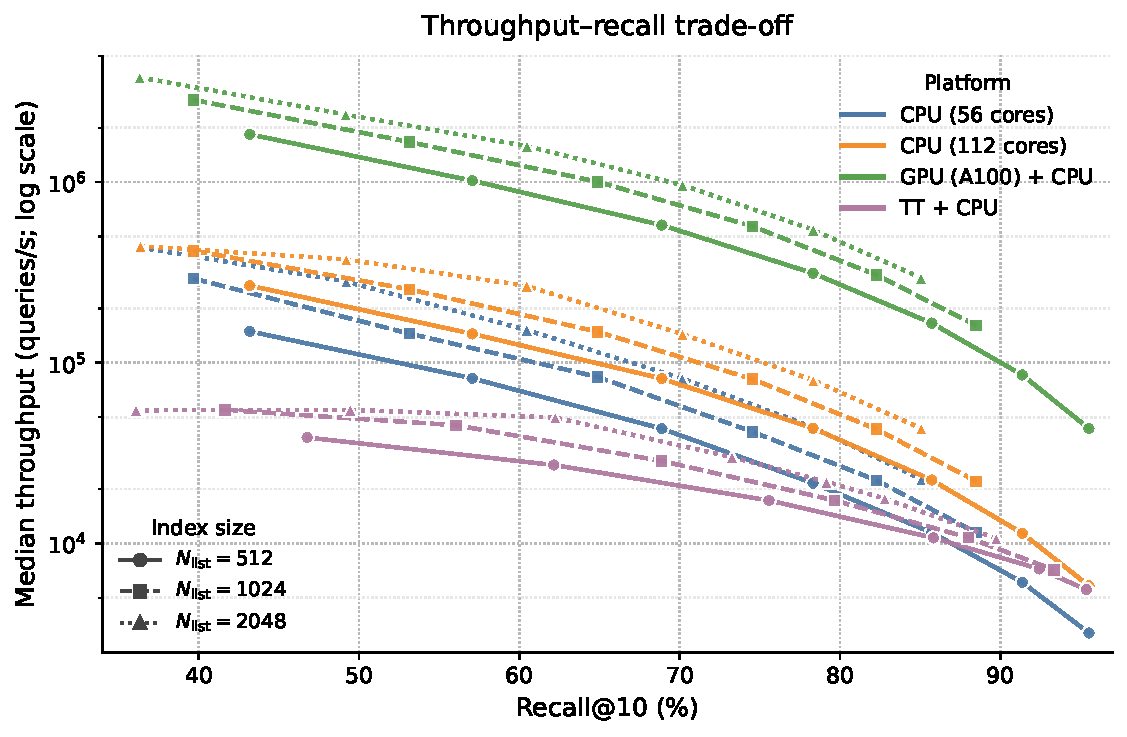
\includegraphics[height=0.78\textheight]{qps_vs_recall.pdf}
\end{frame}

\begin{frame}{Throughput at Matched Recall}
  \centering\footnotesize
  \begin{tabular}{lrrrrrr}
    \toprule
    & \multicolumn{4}{c}{Median QPS} & \multicolumn{2}{c}{Ratio to TT} \\
    \cmidrule(lr){2-5}\cmidrule(lr){6-7}
    Target & CPU 56 & CPU 112 & A100 & TT & CPU 56 & A100 \\
    \midrule
    60\% & 151,858 & 266,184 & 1,583,712 & 49,720 & 3.05 & 31.85 \\
    78\% & 43,864 & 80,075 & 544,703 & 21,907 & 2.00 & 24.86 \\
    88\% & 11,466 & 22,079 & 160,799 & 10,762 & 1.07 & 14.94 \\
    95\% & 3,190 & 5,822 & 43,271 & 5,550 & \textbf{0.57} & 7.80 \\
    \bottomrule
  \end{tabular}\\[3mm]
  \normalsize
  A100 always fastest; Tenstorrent declines more slowly and is \textbf{1.74$\times$} the 56-core CPU at 95\%
\end{frame}

\begin{frame}{Effect of the Batch Union}
  \centering
  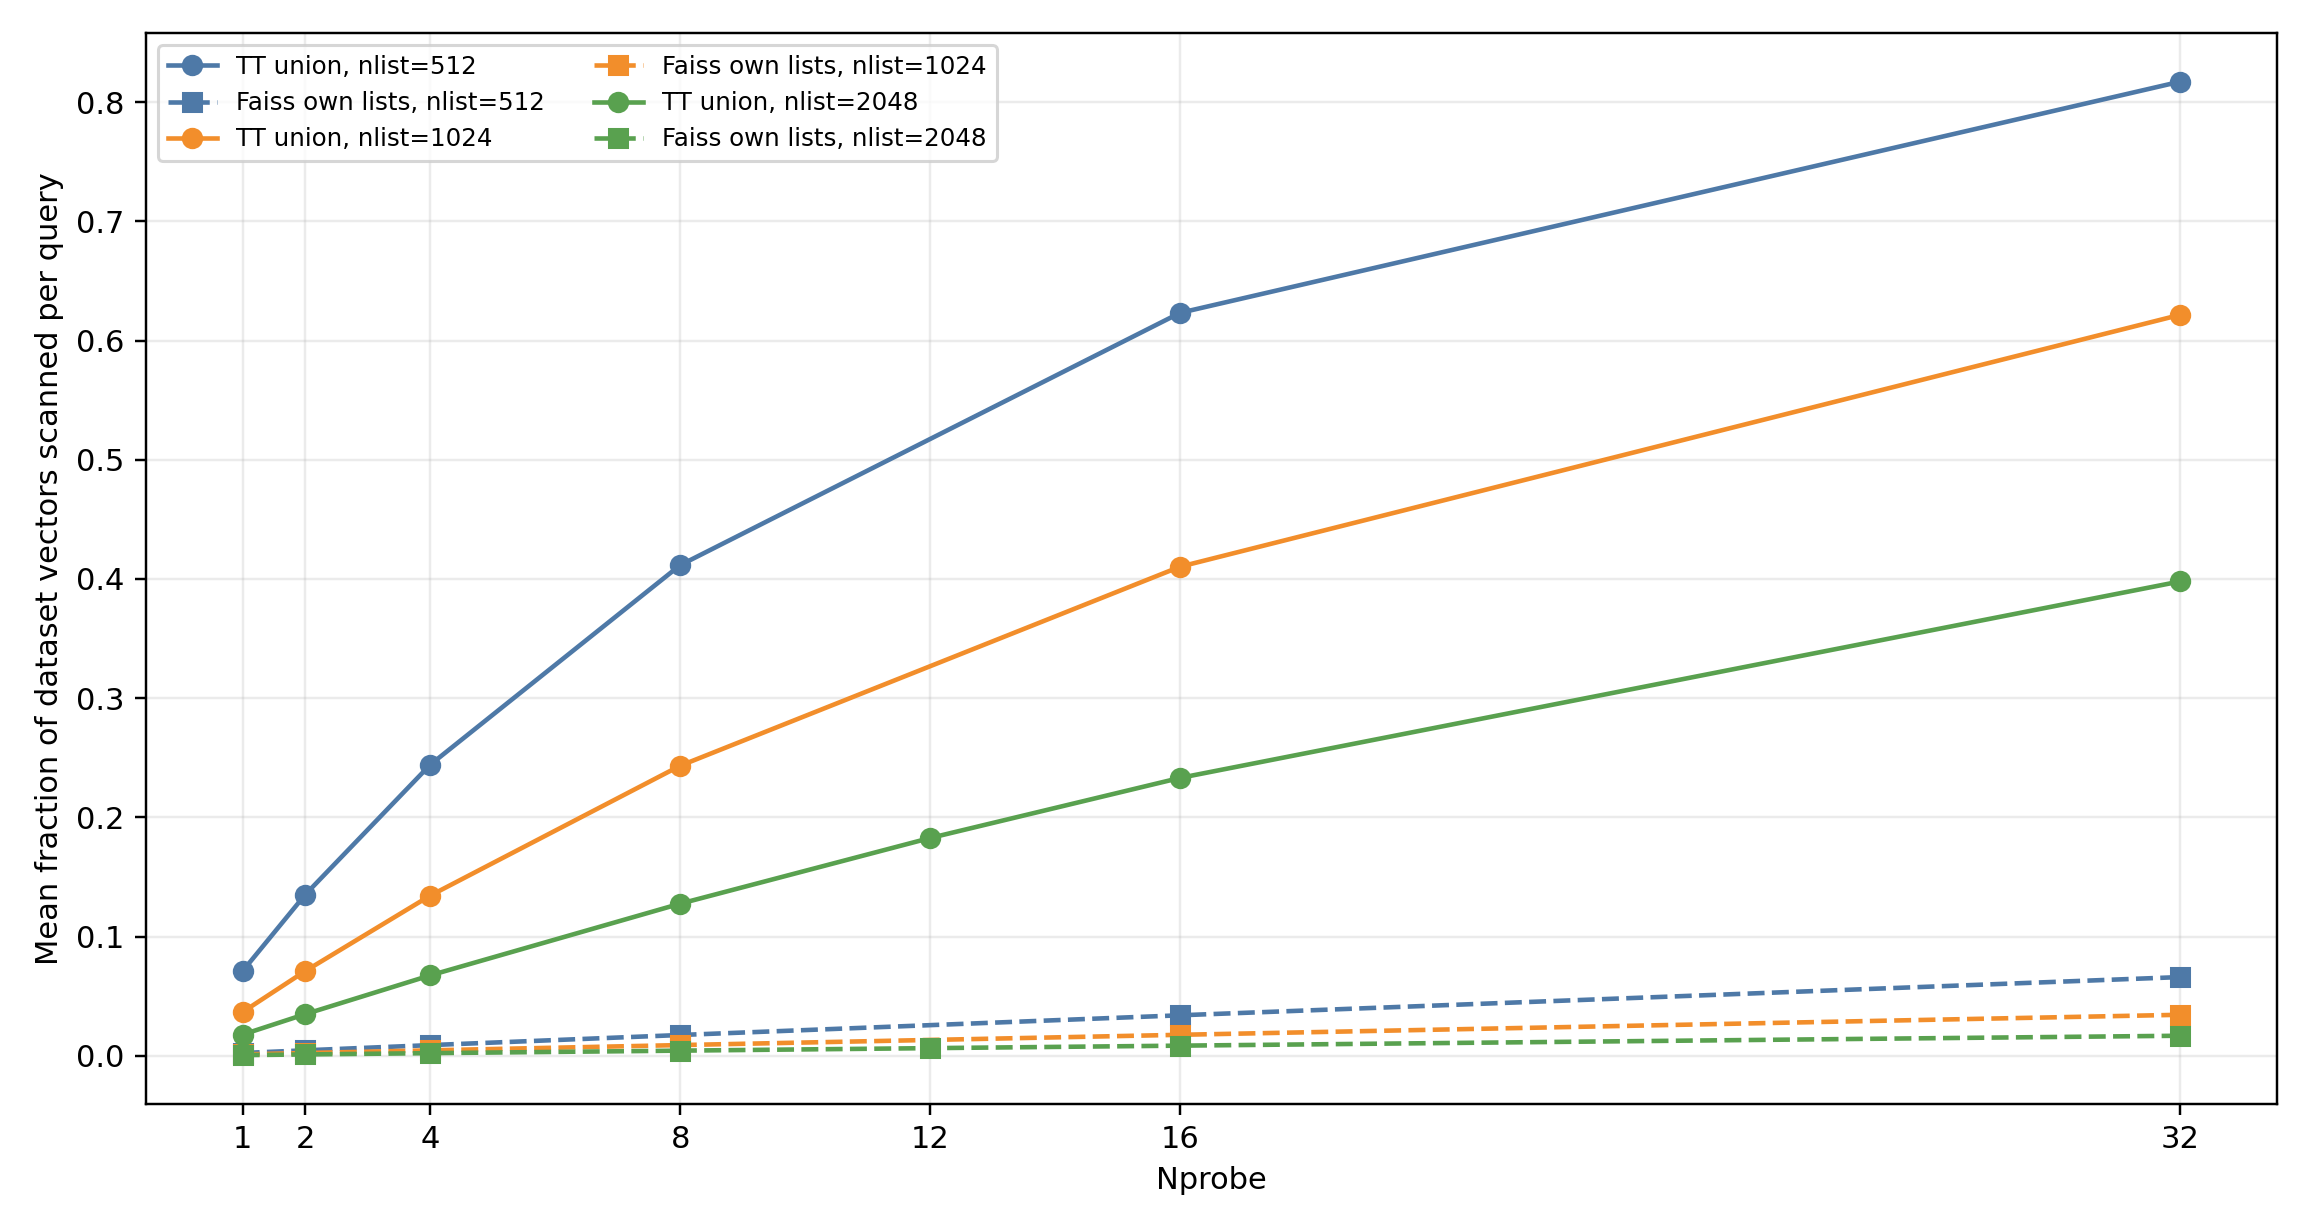
\includegraphics[height=0.66\textheight]{union_scanned_fraction.png}\\[1mm]
  {\footnotesize Each query scans 12--32$\times$ the vectors of its own lists}
\end{frame}

\begin{frame}{Where the Time Goes}
  \begin{columns}
    \column{0.5\textwidth}
    \centering
    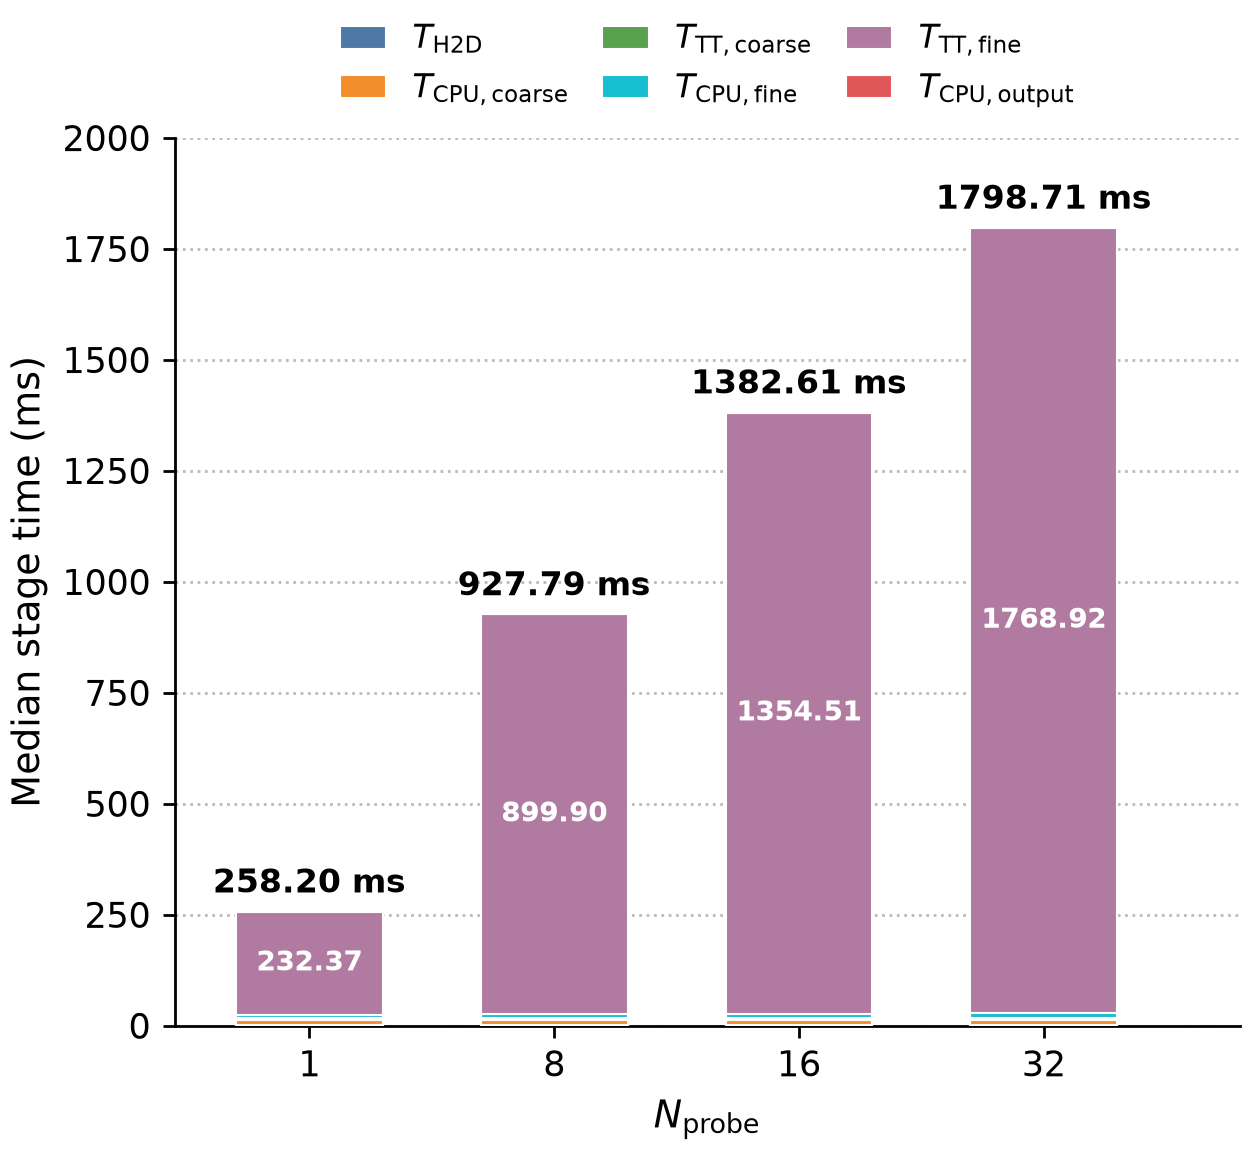
\includegraphics[width=\linewidth]{memcopy_cost_nlist512.png}
    \column{0.5\textwidth}
    \begin{itemize}\footnotesize
      \item $N_{\mathrm{list}}=512$, per 10,000 queries
      \item Fine search: \textbf{90--98\%} of the search time
      \item Host steps and coarse search: under 30\,ms
      \item Memory-bound: about 21 operations per byte vs.\ a balance point of 257
    \end{itemize}
  \end{columns}
\end{frame}

\begin{frame}{Device Timeline}
  \centering
  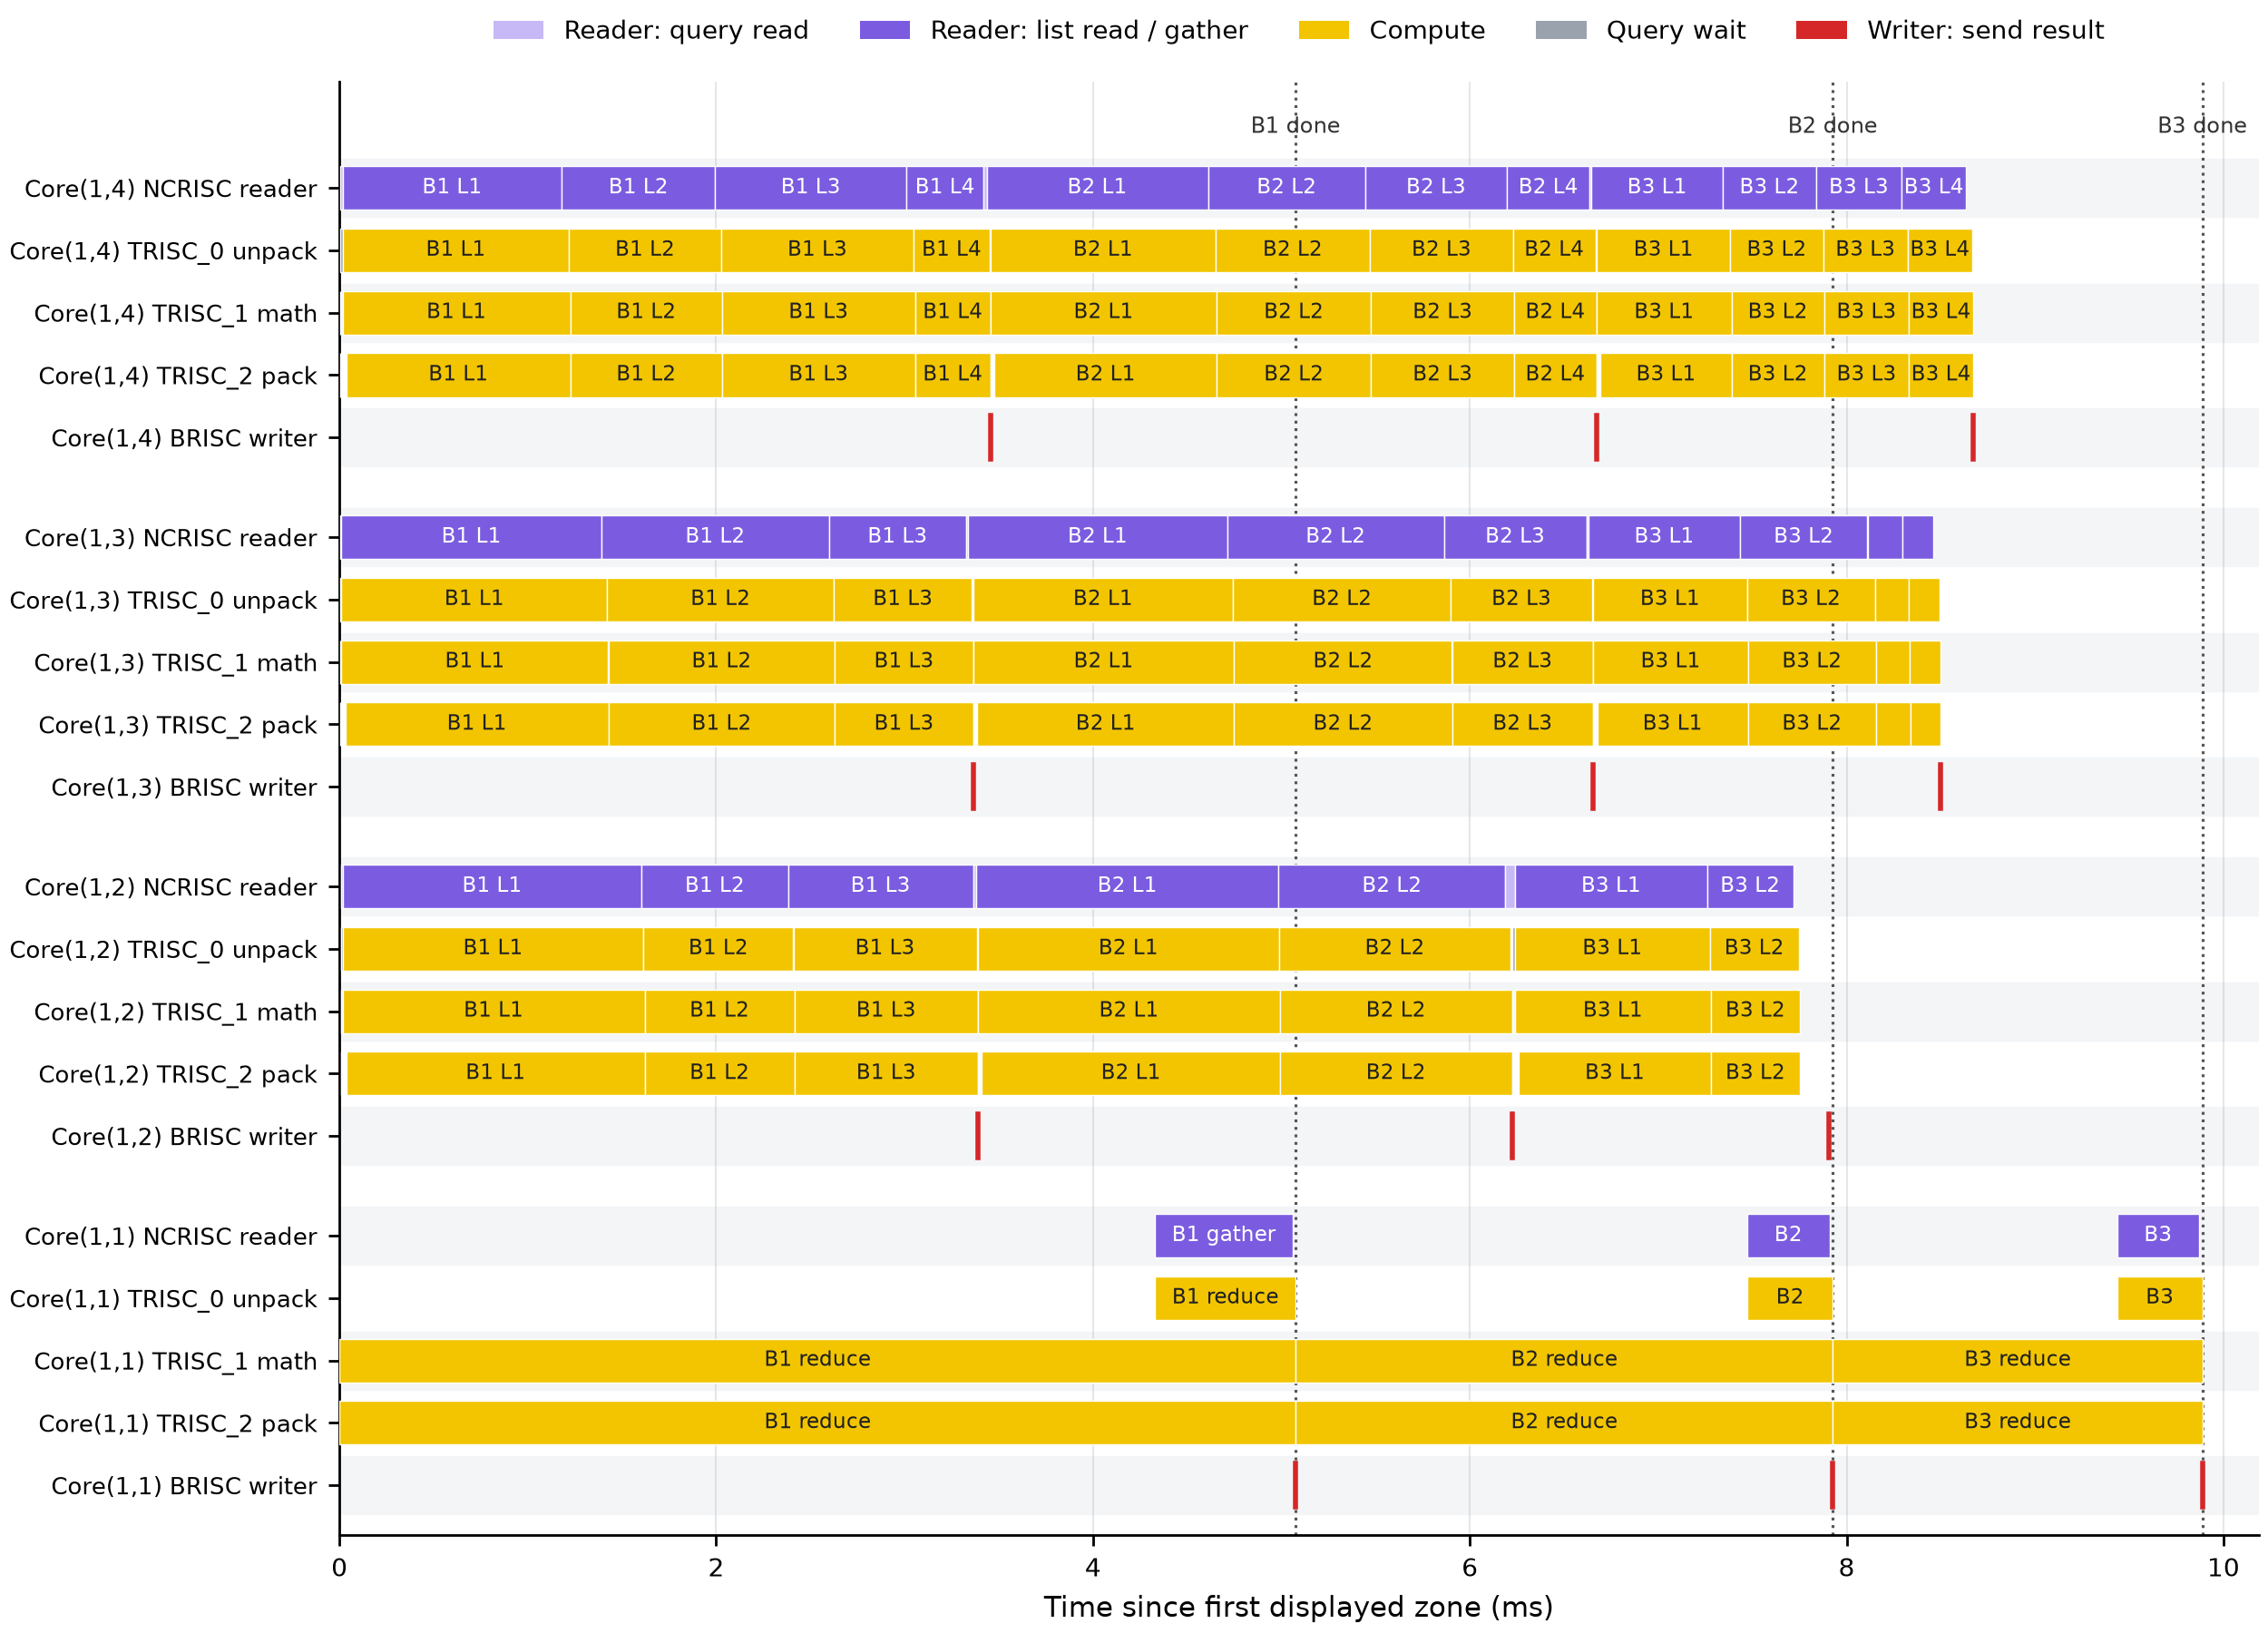
\includegraphics[width=\linewidth,height=0.62\textheight,keepaspectratio]{fine_pipeline_horizontal.png}\\[1mm]
  {\footnotesize Worker imbalance sets batch completion; the aggregation core follows the slowest worker}
\end{frame}

\begin{frame}{Workload Energy}
  \begin{columns}
    \column{0.58\textwidth}
    \centering
    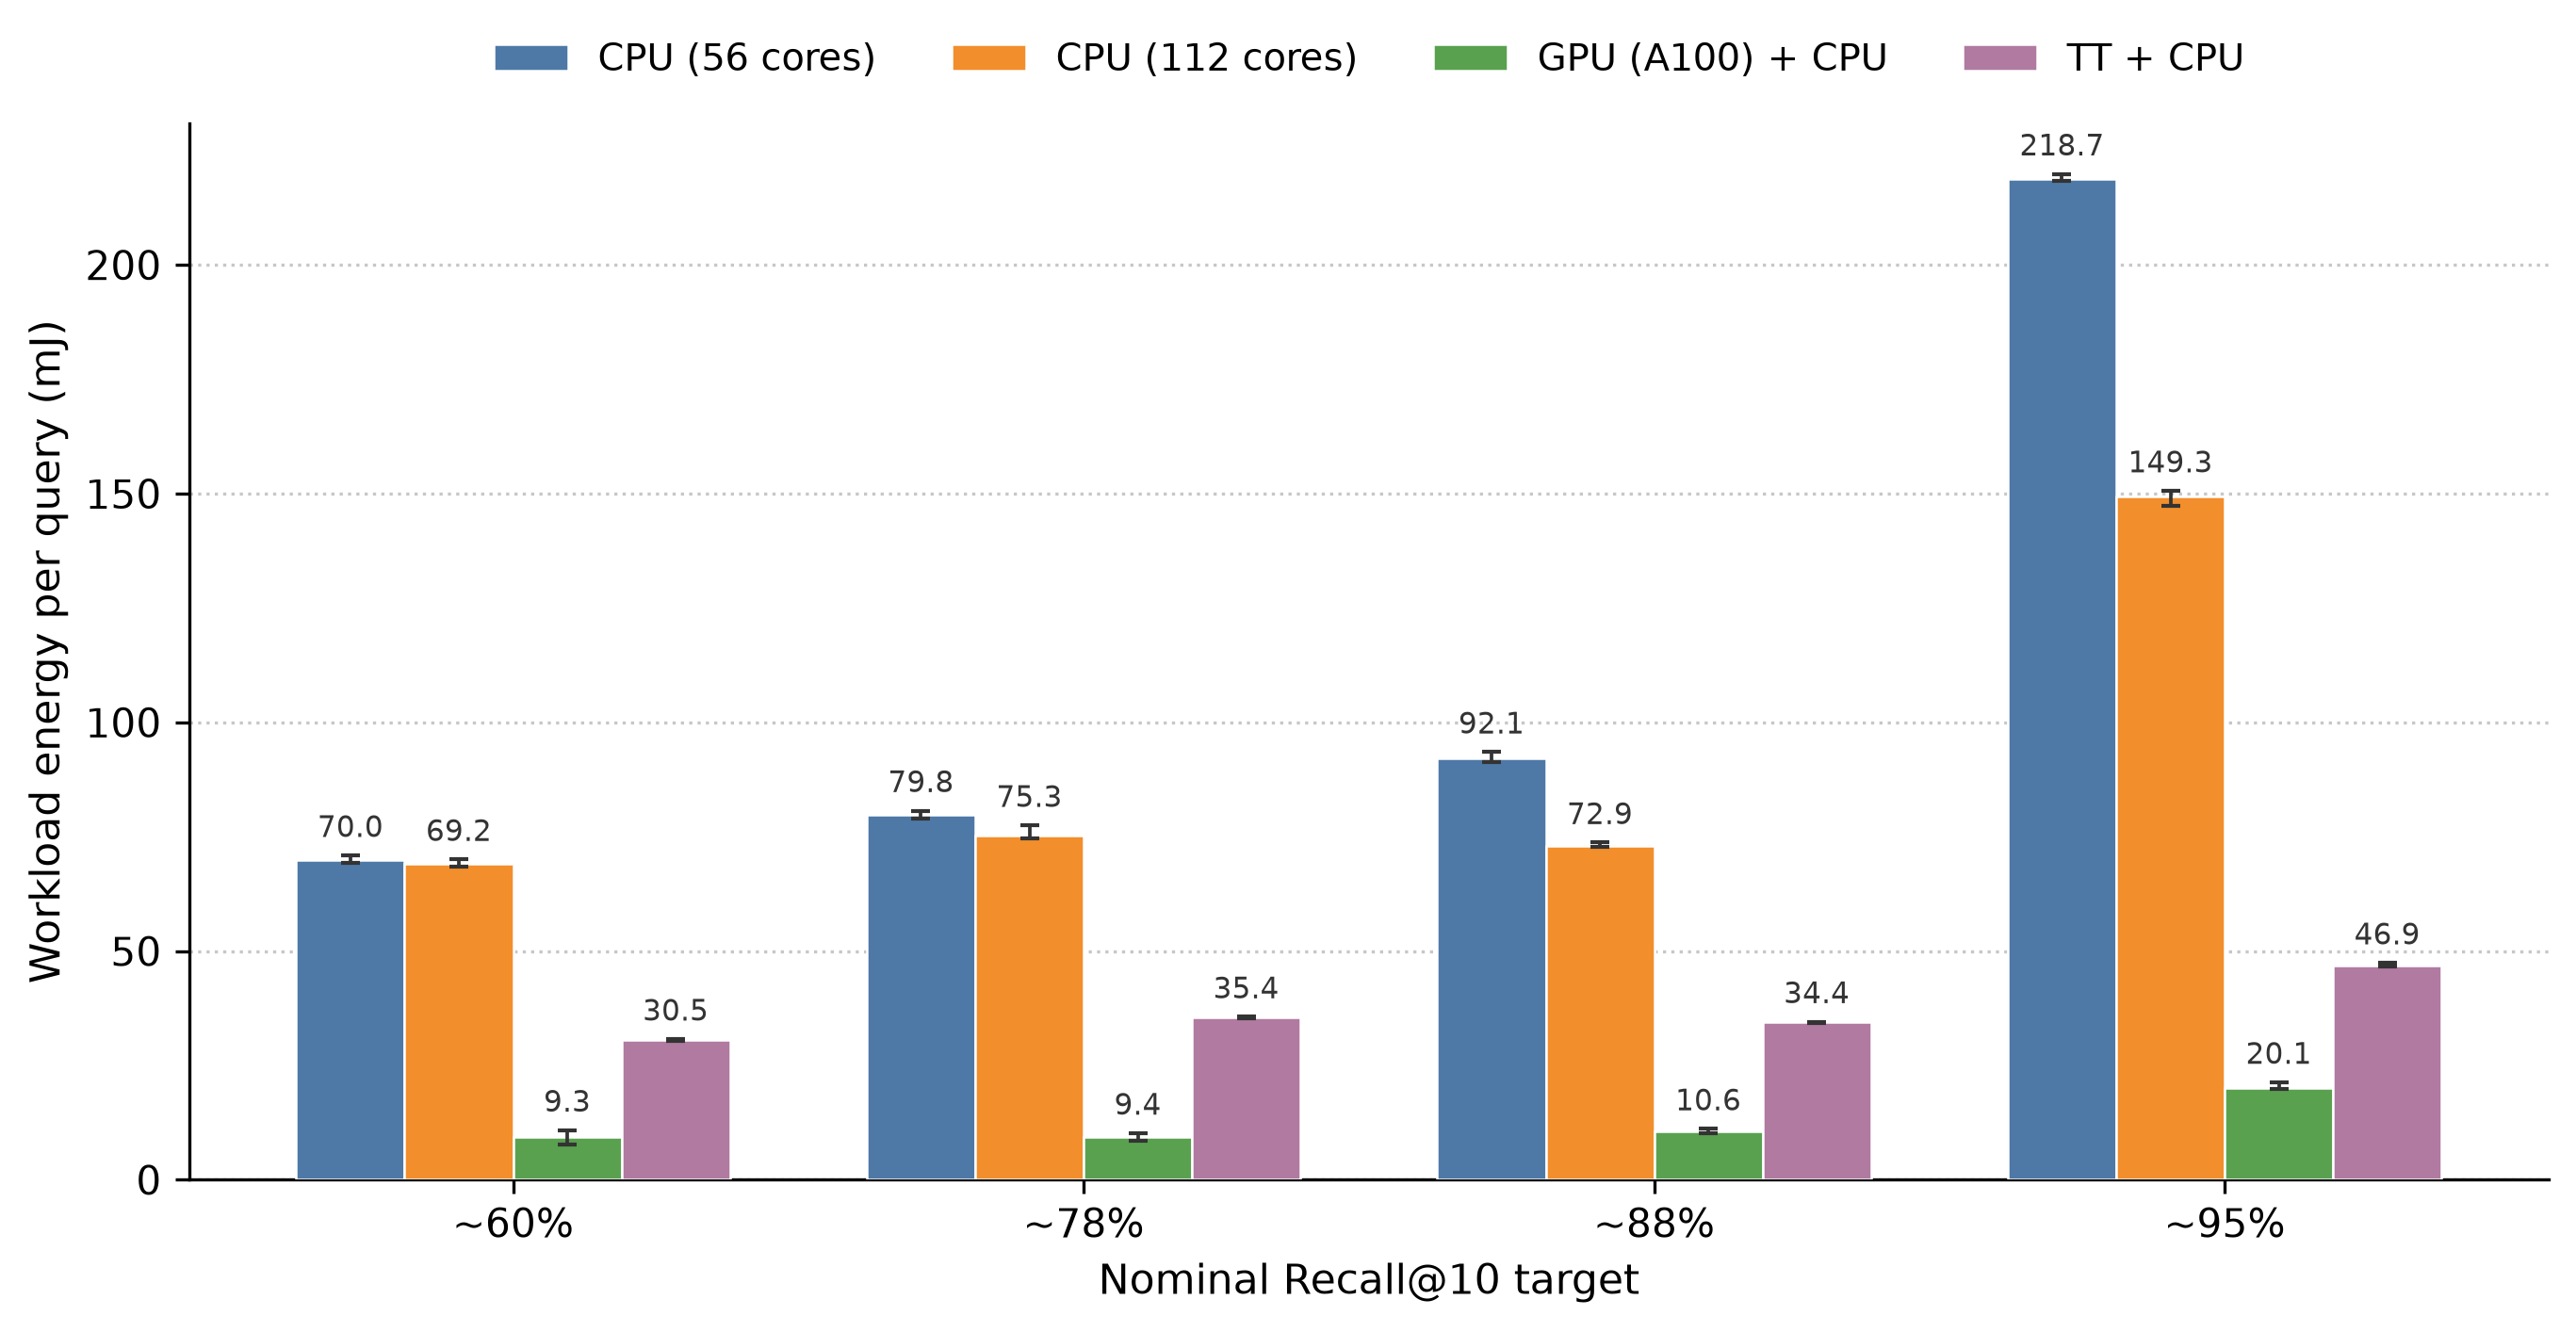
\includegraphics[width=\linewidth]{energy_per_query_recall.png}
    \column{0.42\textwidth}
    \begin{itemize}\footnotesize
      \item A100 system: lowest energy at every target
      \item Tenstorrent system: \textbf{53--79\% less} than the CPUs, 2.3--3.8$\times$ the A100
      \item The Wormhole chip is only \textbf{11--18\%} of its system energy: the host dominates
    \end{itemize}
  \end{columns}
\end{frame}

\begin{frame}{Throughput vs.\ Energy}
  \centering
  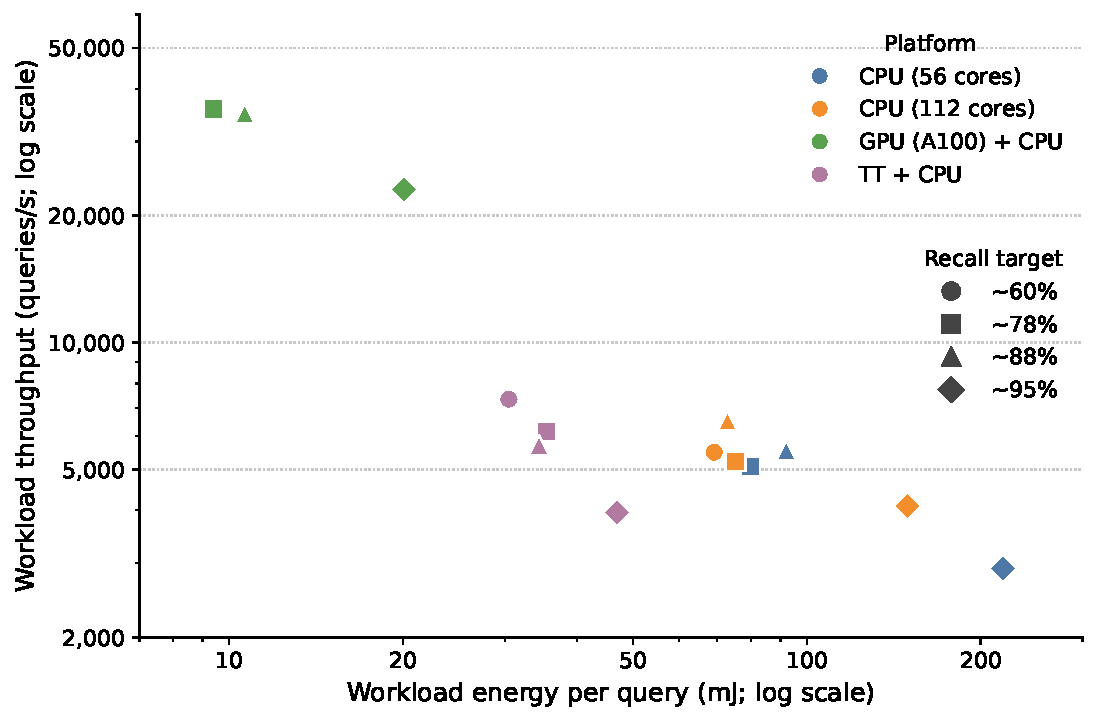
\includegraphics[height=0.78\textheight]{session_throughput_vs_energy.pdf}
\end{frame}

\section{Conclusions}

\begin{frame}{Answers to the Research Questions}
  \begin{enumerate}\small
    \item \textbf{Index:} IVF-Flat fits the tile model best
    \item \textbf{Implementation:} feasible, 95.4\% Recall@10 at 5,550 QPS; the batch union is the main inefficiency
    \item \textbf{Performance:} A100 fastest (7.8--31.9$\times$); Tenstorrent overtakes the 56-core CPU at high recall
    \item \textbf{Energy:} far below the CPUs, above the A100, dominated by the host
  \end{enumerate}
\end{frame}

\begin{frame}{Future Work}
  \begin{itemize}
    \item \textbf{Group queries before batching:} first test at 512 lists, fine search $-57\%$ ($N_{\mathrm{probe}}=16$) and $-42\%$ ($N_{\mathrm{probe}}=32$)
    \item Lighter top-$k$ update per page
    \item Better load balancing across batches and workers
    \item Index structures designed for the device
  \end{itemize}
\end{frame}


\backmatter[notitle]

\end{document}
